
\section{Conceitos de segurança}

    O Computer Security Handbook\cite{nist95}, define segurança computacional como:
    
     \begin{quote}
        ``A proteção oferecida a um sistema de informações automatizado para atingir os objetivos aplicáveis de preservar a integridade, a disponibilidade e a confidencialidade dos recursos do sistema de informações (incluindo \textit{hardware}, \textit{software}, \textit{firmware}, informações / dados e telecomunicações).''
     \end{quote}
     
     Stallings escreve em seu livro \cite{cryptograpy_and_network_stallings} que esta definição introduz os três objetivos chaves da segurança computacional, que estão descritos a seguir:
        
        \begin{itemize}
            \item \textbf{Confidencialidade:} assegura que uma informação privada ou confidencial não estará disponível para indivíduos não autorizados, e que o indivíduo tem controle sob suas informações;
            \item \textbf{Integridade:} assegura que as informações e as aplicações são modificadas somente por indivíduos autorizados, e que os sistemas sejam executados de forma que não haja manipulações por terceiros;
            \item \textbf{Disponibilidade:} Assegura que os sistemas estão prontamente sendo executados e que os serviços não são negados para usuários autorizados.
        \end{itemize}

    \subsection{Criptografia}
    
    A criptografia é o componente mais importante do \textit{blockchain}.A criptografia é certamente um campo de pesquisa em si mesmo, e é baseada em técnicas matemáticas. Houve muitas falhas relatadas em carteiras e trocas de informações devido ao \textit{design} mais fraco ou implementações criptográficas frágeis \cite{beginnig_blockchain_bikramaditya}.
    
    Qualquer informação na forma de uma mensagem de texto, dados numéricos ou um programa de computador pode ser chamada de texto claro. A ideia é cifrar o texto claro usando um algoritmo de cifração/decifração e uma chave que produza o texto cifrado, este último se tornando uma versão protegida do texto claro em relação a confidencialidade. O texto cifrado pode então ser transmitido ao destinatário pretendido, que o decifra usando o algoritmo de decifração e a chave para obter o texto simples.\cite{beginnig_blockchain_bikramaditya}
    
    Em geral, existem dois tipos de criptografia: criptografia de chave simétrica e criptografia de chave assimétrica. A seguir será explicado cada um desses tipos.

        \subsubsection{Modelo de criptografia simétrica}
        
            Um sistema de criptografia simétrica é um sistema criptográfico no qual a cifração e a decifração são executadas usando a mesma chave. Também é conhecido como criptografia convencional. A criptografia simétrica transforma o texto claro em texto cifrado usando uma chave secreta e um algoritmo de cifração. Usando a mesma chave e um algoritmo de decifração, o texto original é recuperado do texto cifrado.\cite{cryptograpy_and_network_stallings}
            
            Assume-se que é impraticável decifrar uma mensagem com base no texto cifrado e no conhecimento do algoritmo de cifração/ decifração. Em outras palavras, não é necessário manter o algoritmo secreto; precisa-se manter apenas o segredo da chave. Esse recurso de criptografia simétrica é o que o torna viável para uso generalizado. Com o uso de criptografia simétrica, o principal problema de segurança é manter o sigilo da chave \cite{cryptograpy_and_network_stallings}.
            
            A Figura \ref{fig:imagem_criptografia_simetrica} representa como é o funcionamento da criptografia simétrica. Na figura, existe a diferenciação de dois canais de comunicação, onde o canal considerado inseguro é utilizado para transmitir o texto que foi cifrado sem prejuízos a sua segurança; e um canal considero seguro para transmitir a chave utilizada para cifrar o texto e que também será utilizada para decifrar o mesmo e recuperar o texto em claro.
            
            \begin{figure}[h]
                 \centering
                 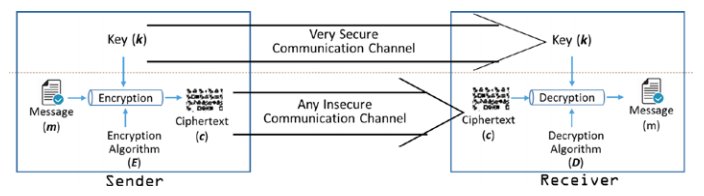
\includegraphics[scale=0.6]{figuras/capitulo_2/criptografia_simetrica.png}
                 \caption{Criptografia Simétrica - Imagem retirada de \cite{beginnig_blockchain_bikramaditya}.}
                 \label{fig:imagem_criptografia_simetrica}
            \end{figure}
            
            A criptografia de chave simétrica existe em duas variantes: \textit{stream ciphers} e \textit{block ciphers} \cite{beginnig_blockchain_bikramaditya}.
            
            Um \textit{stream ciphers} ou \textbf{cifra de fluxo} é a variante que cifra um fluxo de dados digital, um bit ou um byte de cada vez. Se o fluxo de chaves criptográficas for aleatório, essa cifra é inquebrável por qualquer outro meio que não seja a aquisição do fluxo de chaves. No entanto, o fluxo de chaves deve ser fornecido aos dois usuários antecipadamente por meio de um canal independente e seguro. Isso introduz problemas logísticos insuperáveis se o tráfego de dados pretendido for muito grande \cite{cryptograpy_and_network_stallings}.
            
            Consequentemente, por razões práticas, o gerador de fluxo de bits deve ser implementado como um procedimento algorítmico, de modo que o fluxo de bits criptográfico possa ser produzido por ambos os usuários. Nesta abordagem (Figura \ref{fig:imagem_stream_cipher}), o gerador de fluxo de bits é um algoritmo controlado por chave e deve produzir um fluxo de bits criptograficamente fortes. Agora, os dois usuários precisam compartilhar apenas a chave geradora, e cada um pode produzir o fluxo de chaves \cite{cryptograpy_and_network_stallings}.
        
            
                \begin{figure}[h]
                     \centering
                     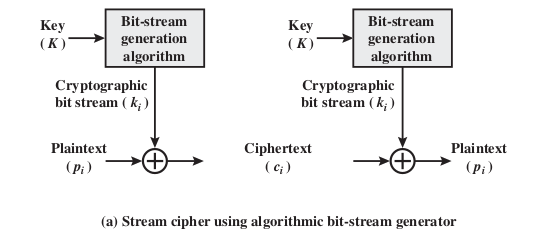
\includegraphics[scale=0.7]{figuras/capitulo_2/stream_cipher_generator.png}
                     \caption{Cifrador de fluxo usando algoritmo gerador de fluxo de bits - Imagem retirada de \cite{cryptograpy_and_network_stallings}.}
                     \label{fig:imagem_stream_cipher}
                \end{figure}
        
            Um \textit{block cipher} ou \textbf{cifra de bloco} é aquela em que um bloco de texto simples é tratado como um todo e usado para produzir um bloco de texto cifrado de comprimento igual. Normalmente, um tamanho de bloco de 64 ou 128 bits é usado. Como ocorre com uma cifra de fluxo, os dois usuários compartilham uma chave de criptografia simétrica (Figura \ref{fig:imagem_block_cipher}).

                \begin{figure}[h]
                     \centering
                     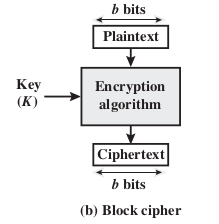
\includegraphics[scale=0.7]{figuras/capitulo_2/block_cipher.png}
                     \caption{Cifrador de Bloco- Imagem retirada de \cite{cryptograpy_and_network_stallings}.}
                     \label{fig:imagem_block_cipher}
                \end{figure}
            
            
        \subsubsection{Modelo de criptografia assimétrico}
        
                Criptografia de chave assimétrica, também conhecida como criptografia de chave pública, é um conceito introduzido por Diffie e Hellman. Com essa técnica, eles resolveram o problema da distribuição de chaves em um sistema de criptografia simétrica, introduzindo também a possibilidade da criação de assinaturas digitais \cite{beginnig_blockchain_bikramaditya}.
                
                Antes de prosseguir, deve-se falar sobre um grande equívoco comum em relação a criptografia de chave pública. Esse equívoco é que a criptografia de chave pública é mais segura do que a criptografia simétrica. De fato, a segurança de qualquer esquema de criptografia depende do tamanho da chave e do trabalho computacional envolvido em quebrar uma cifra. Não há nada em princípio sobre criptografia simétrica ou de chave pública assimétrica que a torne superior a outra do ponto de vista da resistência à criptoanálise  \cite{cryptograpy_and_network_stallings}.

                A criptografia assimétrica é um sistema criptográfico na qual a cifração
                e a decifração são realizadas usando as diferentes chaves - uma chave pública e uma chave privada. A criptografia assimétrica transforma o texto claro em texto cifrado usando uma das duas chaves e um algoritmo de criptografia. Usando a chave emparelhada e um algoritmo de decifração, o texto original é recuperado a partir do texto cifrado. A criptografia assimétrica pode ser usada para confidencialidade, autenticação, ou ambos \cite{cryptograpy_and_network_stallings}.

                A Figura \ref{fig:public_private_encryption} explica como um remetente criptografa o texto claro usando a chave pública de um destinatário, que gera o texto cifrado, que será transmitido pela rede para o receptor. Uma vez que chegue ao receptor, o texto pode ser decifrado usando a chave privada do receptor. Desta forma, a chave privada permanece no lado do receptor e não há necessidade de compartilhar chaves, a fim de realizar a cifração e a decifração, que é o caso da criptografia simétrica \cite{mastering_blockchain}.

                    \begin{figure}[h]
                         \centering
                         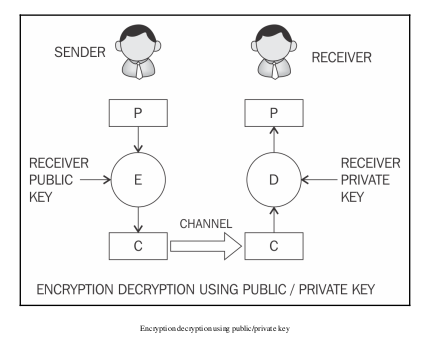
\includegraphics[scale=0.6]{figuras/capitulo_2/public_private_encryption.png}
                         \caption{Criptografia e descriptografia usando chave público/privada - Imagem retirada de \cite{mastering_blockchain}.}
                         \label{fig:public_private_encryption}
                    \end{figure}
                    
                    
                A Figura \ref{fig:public_private_signature} mostra como a criptografia de chave pública pode ser usada para verificar a integridade da mensagem recebida pelo receptor. Nesse modelo, o remetente assina os dados usando sua chave privada e transmite a mensagem para o receptor. Quando a mensagem é recebida no lado do receptor, pode ter sua integridade verificada através do processamento com a chave pública do remetente. Observe que não há busca de confidencialidade/sigilo neste modelo \cite{mastering_blockchain}. Este modelo é usado apenas para fins de autenticação e validação de mensagem.
                    
                    \begin{figure}[h]
                         \centering
                         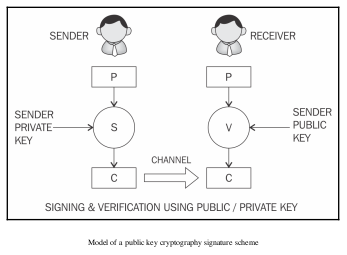
\includegraphics[scale=0.7]{figuras/capitulo_2/public_private_signature.png}
                         \caption{Modelo de esquema assinatura por criptografia de chave pública - Imagem retirada de \cite{mastering_blockchain}.}
                         \label{fig:public_private_signature}
                    \end{figure}
                    
    \subsection{Funções Hash}
        
        Funções hash são funções criptográficas primitivas matemáticas e são parte integrante da estrutura de dados do blockchain. Elas são amplamente utilizadas em muitos protocolos criptográficos, aplicativos de segurança da informação, como assinaturas digitais e códigos de autenticação de mensagens (MACs)  \cite{beginnig_blockchain_bikramaditya}.
        
        Uma função hash H aceita um bloco de comprimento variável de dados M como entrada e produz um valor de hash de tamanho fixo h = H (M). Uma boa função de hash tem a propriedade de que os resultados da aplicação da função a um grande conjunto de entradas produzirá saídas uniformemente distribuídas e aparentemente aleatórias. Em termos gerais, o objetivo principal de uma função hash é a integridade dos dados. Uma mudança em qualquer bit ou bits em M resulta, com alta probabilidade, em uma mudança no hash calculado \cite{cryptograpy_and_network_stallings}.
        
        O tipo de função hash necessária para aplicativos de segurança é chamada de \textbf{função hash criptográfica}. Uma função hash criptográfica é um algoritmo para o qual é computacionalmente inviável (porque nenhum ataque é significativamente mais eficiente que a força bruta) para encontrar (a) um objeto de dados que mapeia para um resultado de hash pré-especificado (a propriedade unidirecional) ou (b) dois objetos de dados que mapeiam para o mesmo resultado de hash (a propriedade livre de colisão). Devido a essas características, as funções hash costumam ser usadas para determinar se os dados foram alterados ou não \cite{cryptograpy_and_network_stallings}.

        A Figura \ref{fig:hash_function} mostra o funcionamento geral de uma função hash criptográfica. Normalmente, a entrada é preenchida com um inteiro múltiplo de algum comprimento fixo (por exemplo, 1024 bits) e o preenchimento inclui o valor do comprimento da mensagem original em bits. O campo de comprimento é uma medida de segurança para aumentar a dificuldade de um invasor para produzir uma mensagem alternativa com o mesmo valor de hash \cite{cryptograpy_and_network_stallings}.
    
                \begin{figure}[h]
                     \centering
                     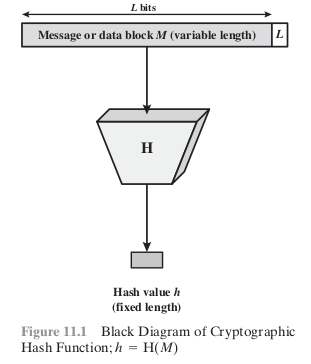
\includegraphics[scale=0.5]{figuras/capitulo_2/hash_function.png}
                     \caption{Diagrama de função de hash criptográfica; h = H(M) - Imagem retirada de \cite{cryptograpy_and_network_stallings}.}
                     \label{fig:hash_function}
                \end{figure}
                
        Uma das mais antigas funções de hash, ou função de compressão, é a função hash MD4, que pertence à família message digest (MD). Entre os membros da família MD temos MD5 e MD6, e muitas outras variantes do MD4, como o RIPEMD. A família de algoritmos MD produz um resumo de mensagens de 128 bits consumindo blocos de 512 bits. Eles foram amplamente utilizados como checksums para verificar a integridade dos dados \cite{beginnig_blockchain_bikramaditya}.
        
        Outra família de funções hash amplamente utilizada é a \textbf{Secure Hash Algorithm (SHA)}. Existem basicamente quatro algoritmos nessa família: SHA-0, SHA-1, SHA-2 e SHA-3 \cite{beginnig_blockchain_bikramaditya}.

    
        \subsubsection{Ponteiros Hash}
        
            Um \textbf{ponteiro de hash (hash pointer)} é um hash criptográfico apontando para um bloco de dados, onde o ponteiro de hash é o hash do próprio bloco de dados (Figura \ref{fig:hash_pointer}). Ao contrário das listas vinculadas que apontam para o próximo bloco para que você possa chegar até ele, os ponteiros de hash apontam para o bloco de dados anterior e fornecem uma maneira de verificar se os dados não foram adulterados  \cite{beginnig_blockchain_bikramaditya}.
            
                \begin{figure}[h]
                     \centering
                     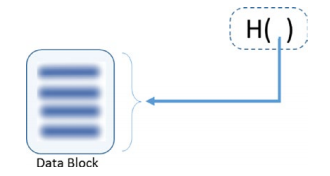
\includegraphics[scale=0.8]{figuras/capitulo_2/hash_pointer.png}
                     \caption{Ponteiro Hash para um bloco de dados - Imagem retirada de \cite{beginnig_blockchain_bikramaditya}.}
                     \label{fig:hash_pointer}
                \end{figure}
            
            O objetivo do ponteiro de hash é construir uma cadeia de blocos que pode ser considerada como uma fonte única de verdade. Seu funcionamento se baseia no fato que o hash do bloco anterior é armazenado no cabeçalho do bloco atual e o hash do bloco atual com o cabeçalho do bloco será armazenado no cabeçalho do próximo bloco. Isso cria uma cadeia de blocos como podemos ver na Figura \ref{fig:blocks_linked_hash_pointers}  \cite{beginnig_blockchain_bikramaditya}.
            
                \begin{figure}[h]
                     \centering
                     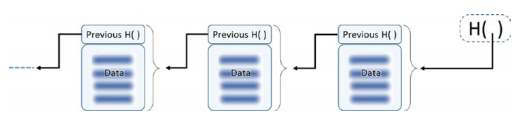
\includegraphics[scale=0.8]{figuras/capitulo_2/blocks_linked_hash_pointers.png}
                     \caption{Blocos encadeados ligados por ponteiros hash - Imagem retirada de \cite{beginnig_blockchain_bikramaditya}.}
                     \label{fig:blocks_linked_hash_pointers}
                \end{figure}


        \subsubsection{Merkle Trees}
  
            Uma Árvore Merkle, também conhecida como uma árvore hash binária, é uma estrutura de dados usada para resumir e verificar eficientemente a integridade de grandes conjuntos de dados. Árvores Merkle são árvores binárias contendo hashes criptográficos. O termo árvore é usado na ciência da computação para descrever uma estrutura de dados de ramificação, mas essas árvores geralmente são exibidas de cabeça para baixo com a raiz na parte superior e as folhas na parte inferior de um diagrama.\cite{mastering_blockchain_andreas}
            
            Uma típica Árvore Merkle pode ser representada como na Figura \ref{fig:merkle_tree_representation}.
        
                \begin{figure}[h]
                     \centering
                     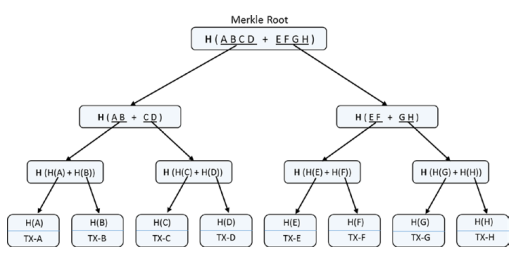
\includegraphics[scale=0.7]{figuras/capitulo_2/merkle_tree_representation.png}
                     \caption{Representação de uma Árvore de Merkle - Imagem retirada de \cite{beginnig_blockchain_bikramaditya}}
                     \label{fig:merkle_tree_representation}
                \end{figure}

            Semelhante à estrutura de dados do ponteiro hash, a árvore Merkle também é resistente à adulteração. A adulteração em qualquer nível da árvore não corresponderia ao hash armazenado em um nível acima na hierarquia e também até o nó raiz. É realmente difícil para um adversário alterar todos os hashes da árvore inteira. Também garante a integridade da ordem das transações. Se você alterar apenas a ordem das transações, também os hashes na árvore até a raiz Merkle serão alterados.\cite{beginnig_blockchain_bikramaditya}


\section{Sistemas Distribuídos}

    Diversas definições de sistemas distribuídos são apresentadas na literatura, onde estas variam de acordo com o contexto em que está é apresentada. Para o propósito deste trabalho, pode-se dizer que: “Um sistema distribuído é uma coleção de elementos computacionais autônomos que para os usuários parecem ser um único sistema coerente. Um elemento computacional, normalmente chamado de nó, pode ser tanto um dispositivo de hardware ou um processo de software” \cite{sistemas_distribuidos_tanembaum}.

    Um nó pode ser definido como um “jogador individual”, onde em um sistema distribuído todos os nós tem a capacidade de enviar e receber mensagem entre eles. Estes nós podem ser honestos, faltantes ou maliciosos e podem ter sua própria memória e processador. Um nó que apresenta um comportamento arbitrário também é chamado de Nó Bizantino \cite{mastering_blockchain}.

    O maior desafio em sistemas distribuídos é a coordenação entre esses nós e a tolerância a falha. Pois mesmo que um determinado nó apresente uma falha de conexão durante um período de tempo ou caso um nó não esteja presente na rede, a mesma deve tolerar estes problemas e continuar seu funcionamento de forma a alcançar o objetivo estabelecido. Estes sistemas 
    são considerados tão desafiadores que seus conceitos são comumente estudados levando em consideração resultados decorrentes do Teorema de CAP.

    \subsection{Teorema de CAP}

        Este teorema, também conhecido como \textit{Brewer's Theorem}, foi introduzido inicialmente em 1998 por Eric Brewer e provado como um teorema em 2002 por Seth Gilbert e Nancy Lynch.

        O teorema determina que um sistema distribuído não pode ter Consistência (\textit{Consistency}), Disponibilidade (\textit{Availability}) e Tolerância a Partição (\textit{Partition}) de forma simultânea \cite{brewer_distributed}. A seguir cada um destes é explicado de forma rápida:

        \begin{itemize}
            \item \textbf{Consistência:} é a propriedade que garante que todos os nós em um sistema distribuído possuem pelo menos uma cópia atualizada dos dados;
            \item \textbf{Disponibilidade:} essa propriedade garante que um sistema está disponível, acessível para uso, e aceitando novas requisições e respondendo-as;
        com os dados sem nenhuma falha e sempre quando é requisitado;
            \item \textbf{Tolerância a Partição:} garante que caso um grupo de nós falhe, o sistema distribuído ainda continua a operar corretamente.
        \end{itemize}

    \subsection{O Problema dos generais bizantinos}
    

           Nos primórdios da computação comercial, por volta de 1980, cientistas da computação começaram a examinar a confiabilidade e os computadores. Foi estabelecido que um sistema de computador confiável deveria ser capaz de lidar com a falha de um ou mais de seus componentes. Um componente com falha pode exibir um tipo de comportamento negligenciado e problemático, ou seja, enviar informações conflitantes para diferentes partes do sistema. O problema de lidar com esse tipo de falha é expresso abstratamente como o Problema dos Generais Bizantinos, do artigo acadêmico de 1982 de Leslie Lamport, Robert Shostak e Marshall Pease  \cite{blockchain_pratical_guide}.
           
           O problema dos generais bizantinos é construído em torno do seguinte enredo no artigo de \citeonline{byzantine_problem_article}: várias divisões do exército bizantino estão acampados ao redor de uma cidade inimiga e cada uma dessas divisões é comandada por um general, onde estes podem se comunicar somente por meio de mensagens. Após observar o inimigo estes generais precisam chegar a um consenso em relação a um plano único de ataque, porém alguns destes generais podem ser traidores tentando fazer com que generais leais não cheguem a um acordo. Para que este acordo seja realizado, estes generais precisam de um algoritmo que garanta que todos os generais leais decidam sobre o mesmo plano de ação e que um pequeno número de generais traidores não façam com que os generais leais adotem um plano de ação ruim.
           
            Na analogia, os generais são coletivamente conhecidos como processos, o general que inicia a comunicação com os outros é o processo de origem e as ordens enviadas aos outros processos são mensagens. Generais traidores são processos defeituosos, e generais leais são processos corretos. A ordem para recuar ou atacar é uma mensagem com um único bit de informação: um ou zero. Uma solução para este problema de acordo deve passar por três testes: rescisão, acordo e validade. Conforme aplicado ao problema dos generais bizantinos, \citeonline{blockchain_pratical_guide} define que estes testes avaliam as seguintes características:
    
               \begin{enumerate}
                    \item Uma solução deve garantir que todos os processos corretos cheguem a uma decisão em relação ao valor da ordem que eles receberam;
                    \item Todos os processos corretos devem decidir sobre o mesmo valor da ordem que receberam com os dados sem nenhuma falha e sempre quando é requisitado;
                    \item Se o processo de origem for um processo correto, todos os processos devem decidir sobre o valor que foi original dado pelo processo de origem.
                \end{enumerate}
    
            Em seu artigo \citeonline{byzantine_problem_article} apresentam diferentes soluções que podem ser adotadas para solucionar este problema de consenso entre os generais. Estas abordagens descritas foram utilizadas na concepção da rede Blockchain como insumo para a criação dos diferentes protocolos de consenso utilizados para gerenciar esta rede distribuída.   
    
    
   
\section{Blockchain}

    
    Em 2008 um hacker anônimo (ou um grupo de hackers), utilizando o pseudônimo Satoshi Nakamoto, lançou a primeira moeda totalmente virtual e pouco tempo divulgou um artigo \cite{bitcoin_satoshi}. Esse artigo denominado de \textit{Bitcoin: A Peer-to-Peer Electronic Cash System} detalhava os métodos para o uso de uma rede peer-to-peer para gerar o que era descrito como “um sistema para transações eletrônicas sem abnegar a confiança”.
    
    Nakamoto combinou várias invenções anteriores, como b-money e HashCash para criar um sistema de caixa eletrônico completamente descentralizado que não dependia de uma autoridade central para emissão ou liquidação de moeda e validação de transações. A principal inovação foi usar um sistema de computação distribuída (chamado de algoritmo de “Prova-de-Trabalho”) para conduzir uma “eleição” global a cada 10 minutos, permitindo a rede descentralizada para chegar a um consenso sobre o estado das transações. Isso resolve elegantemente a questão do gasto duplo, em que uma única unidade monetária pode ser gasta duas vezes. Anteriormente, o problema do gasto duplo era uma fraqueza da moeda digital e era resolvido com a compensação de todas as transações por meio de uma central de compensação \cite{mastering_blockchain_andreas}.
    
    O Bitcoin transformou totalmente os conceitos de bancos, dinheiro, processos de pagamentos entre outros; por meio da criação de um único registro digital acessível universalmente chamado de Blockchain. Foi atribuído esse nome de corrente porque mudanças só podem ser realizadas adicionando novas informações ao final, como em uma corrente de ferro, e cada nova adição a esta corrente contém um determinado números de transações.



    \subsection{Definição}
    
    A abstração para o entendimento de sistemas Blockchain é a noção de livro razão, uma invenção desenvolvida pelos renascentistas italianos para suportar escrituração de dupla entrada, um precursor distante das criptomoedas modernas. Um livro contábil é apenas um registro indelével e unificado de transações que ocorrem entre várias partes. Um livro-razão estabelece quais transações aconteceram e a ordem em que essas transações aconteceram. Livros razão são públicos, acessíveis a todas as partes, e devem ser à prova de falsificação: nenhuma das partes pode adicionar, excluir ou modificar as entradas do livro, uma vez gravadas \cite{blockchain_computing_perspective}.
    
    Pode se definir blockchain, em termos técnicos, como: “um blockchain é um ledger distribuído de transações implementadas como dados agrupados em blocos que usam validação criptográfica para vincular os blocos. Cada bloco referencia e identifica o bloco anterior usando uma função de \textit{hashing} que forma uma cadeia ininterrupta (isto é, blockchain)” \cite{blockchain_pratical_guide}.
    
    De um ponto de vista empresarial, podemos caracterizar Blockchain como uma plataforma onde diferentes nós podem realizar troca de valores utilizando transações sem a necessidade de uma terceira parte autenticadora.
    
    
    \subsection{Tipos de Blockchain}
    \label{subsection_tipos_blockchain}

    Quando as pessoas começaram a entender o funcionamento do blockchain, começaram a usá-lo para outros fins: como armazenamento de dados para coisas de valor, identidades, acordos, direitos de propriedade e uma série de outras coisas \cite{blockchain_pratical_guide}. Cada uma dessas possíveis aplicações acaba demandando diferentes características e restrições para seu funcionamento, fazendo com que surgissem diferentes tipos e categorias de blockchain.
    
    Os tópicos a seguir trarão uma pequena descrição sobre alguns dos diferentes tipos de blockchain.
    
    
    \subsubsection{Blockchains Públicos}
    
    Conforme definido pelos criadores originais da tecnologia, um blockchain público é aquele que tem como característica o fato de todos poderem acessar e realizar transações sem uma restrição para que novos nós sejam inseridos na rede; um blockchain onde as transações são incluídas se e somente se forem válidas; um blockchain onde todos podem contribuir para o processo de consenso \cite{blockchain_pratical_guide}.
    
    No blockchain público, em vez de usar um servidor central, o blockchain é assegurado por verificação criptográfica por incentivos para os chamados mineradores (\textit{miners}). Qualquer um pode ser um minerador para agregar e publicar essas transações. No blockchain público, como nenhum usuário é implicitamente confiável para verificar transações, todos os usuários seguem um algoritmo que verifica transações comprometendo recursos de software e hardware para resolver um problema por força bruta resolvendo um tipo de quebra-cabeça criptográfico  \cite{blockchain_pratical_guide}.
    

    \subsubsection{Permissioned ledger}
    
    É um tipo de blockchain no qual os participantes da rede (nós) são conhecidos e já são confiáveis. Os registros autorizados não precisam usar um mecanismo de consenso distribuído. Em vez disso, um protocolo de acordo pode ser usado para manter uma versão compartilhada da verdade em relação ao estado dos registros no blockchain. Também não há exigência de que um \textit{permissioned ledger} seja privado, pois pode ser um blockchain público, mas com controle de acesso regulado \cite{mastering_blockchain}.

    \subsubsection{Private Blockchain}

    Um blockchain totalmente privado é um blockchain no qual as permissões de gravação são mantidas centralizadas em uma organização. Permissões de leitura podem ser públicas ou restritas a uma extensão arbitrária. Aplicações prováveis incluem gerenciamento de banco de dados e auditoria interna para uma única empresa, de modo que a legibilidade pública pode não ser necessária em muitos casos, embora em outros casos a auditabilidade pública seja desejada  \cite{blockchain_pratical_guide}.



    \subsection{Estrutura de um bloco}

        Um bloco é uma estrutura de dados que agrega transações para inclusão no livro razão público, o blockchain. O bloco é feito de um cabeçalho, contendo metadados, seguido por uma longa lista de transações que compõem a maior parte do seu tamanho. O cabeçalho do bloco é de 80 bytes, enquanto o tamanho médio das transações é de pelo menos 250 bytes e um bloco médio contém mais de 500 transações. Um bloco completo, com todas as transações, é, portanto cerca de 1.000 vezes maior que o cabeçalho do bloco \cite{mastering_blockchain_andreas}.

        Um bloco é composto de uma seleção de transações organizadas de forma ordenada para que ocorra um encadeamento lógico. Esse bloco é composto por transações, e também contém uma referência ao bloco anterior. A estrutura do bloco varia de acordo com o tipo e design do Blockchain \cite{mastering_blockchain}.
        
        A Tabela \ref{tabela_estrutura_de_um_bloco} apresenta a estrutura de um bloco de forma geral.
            
        \begin{table}[h]
            \centering
            \caption{A estrutura de um bloco.}
                \begin{tabular}{|l|l|l|}
                \hline
                \multicolumn{1}{|c|}{\textbf{Tamanho}} & \multicolumn{1}{c|}{\textbf{Campo}} & \multicolumn{1}{c|}{\textbf{Descrição}} \\ \hline
                 4 bytes & Tamanho do Bloco & O tamanho do bloco, em bytes, após esse campo \\ \hline
                 80 bytes   & Cabeçalho do Bloco & Os campos do cabeçalho do bloco  \\ \hline
                 1-9 bytes  & Contador da transação & Quantas transações seguem  \\ \hline
                 Variável   & Lista de Transações / Dados   & As transações/dados gravados nesse bloco\\ \hline
                \end{tabular}
            \label{tabela_estrutura_de_um_bloco}
        \end{table}




    \subsection{Cabeçalho de um bloco}

    O cabeçalho do bloco consiste em três conjuntos de metadados do bloco. Primeiro, há uma referência a um hash do bloco anterior, o que conecta esse bloco ao bloco anterior na Blockchain. O segundo conjunto de metadados é composto pelos campos: a dificuldade, o registro de data e hora e o identificador único (contador), onde estes estão relacionadas à concorrência na mineração. A terceira parte dos metadados é a raiz da Árvore de Merkle, uma estrutura de dados usada para resumir eficientemente todas as transações no bloco \cite{mastering_blockchain_andreas}.

    A Tabela \ref{tabela_estrutura_cabecalho_de_um_bloco} apresenta a estrutura de um cabeçalho de um bloco de forma geral.
    

    \begin{table}[h]
        \centering
        \caption{Estrutura do cabeçalho de um bloco.}
        \begin{adjustbox}{width=\textwidth}
            \begin{tabular}{|l|l|l|}
            \hline
            \multicolumn{1}{|c|}{\textbf{Tamanho}} & \multicolumn{1}{c|}{\textbf{Campo}} & \multicolumn{1}{c|}{\textbf{Descrição}} \\ \hline
             4 bytes & Versão   & A versão numérica para controle de atualizações  \\ \hline
             32 bytes & Hash do bloco anterior   & Uma referência ao hash do bloco anterior (pai) na cadeia \\ \hline
             32 bytes & Raiz da Árvore de Merkle    & Um hash da raiz da Árvore de Merkle das transações deste bloco  \\ \hline
             4 bytes  & Timestamp  & O tempo aproximado de criação deste bloco  \\ \hline
             4 bytes  & Dificuldade  & A dificuldade do algoritmo de prova de trabalho para este bloco  \\ \hline
             4 bytes  & Identificador Único  & Um contador usado para o algoritmo de prova de trabalho  \\ \hline
            \end{tabular}
        \end{adjustbox}
        \label{tabela_estrutura_cabecalho_de_um_bloco}
    \end{table}




    \subsection{Block Header Hash e Block Height, identificadores de um bloco}
    
    O identificador primário de um bloco é seu hash criptográfico, uma impressão digital, feita pela aplicação do hash do cabeçalho do bloco duas vezes através do algoritmo SHA256. O hash de 32 bytes resultante é chamado de hash de bloco, mas é mais precisamente o hash de cabeçalho de bloco, porque somente o cabeçalho de bloco é usado para calculá-lo. O hash de bloco identifica um bloco de forma única e inequívoca e pode ser derivado independentemente por qualquer nó simplesmente fazendo hash no cabeçalho do bloco \cite{mastering_blockchain_andreas}.
    
    Uma segunda maneira de identificar um bloco é por sua posição no blockchain, chamado altura do bloco, onde o primeiro bloco criado está na altura 0. Cada bloco subsequente adicionado “no topo” daquele primeiro bloco é uma posição “superior” no blockchain, como caixas empilhadas uma sobre a outra \cite{mastering_blockchain_andreas}.

    Ao contrário do hash do bloco, a altura do bloco não é um identificador exclusivo. Embora um único bloco tenha sempre uma altura de bloco específica e invariante, o inverso não é verdadeiro, a altura do bloco nem sempre identifica um único bloco. Dois ou mais blocos podem ter a mesma altura de bloco, competindo pela mesma posição no blockchain.
    
    
    
    \subsection{Consenso no blockchain}

        O consenso é um processo de concordância entre nós que não possuem confiança mútua em um estado final de dados. Para alcançar consenso, diferentes algoritmos podem ser usados. É fácil chegar a um acordo entre dois nós (por exemplo, em sistemas cliente-servidor), mas quando vários nós participam de um sistema distribuído e precisam concordar em um único valor, torna-se muito difícil chegar a um consenso. Esse conceito de alcançar consenso entre vários nós é conhecido como consenso distribuído \cite{mastering_blockchain}.
        
        Um mecanismo de consenso é um conjunto de etapas tomadas por todos, ou a maioria dos nós, para chegar a um acordo sobre um estado ou valor proposto. Por mais de três décadas este conceito tem sido pesquisado por cientistas da computação na indústria e na academia. Mecanismos de consenso recentemente entraram no centro das atenções e ganharam muita popularidade com o advento do bitcoin e blockchain \cite{mastering_blockchain}.
        
        Cada blockchain tem seus próprios algoritmos para criar um acordo dentro de sua rede nas entradas adicionadas, onde o processo de entrada pode ser visualizado na Figura \ref{fig:blockchain_work_dummies}. Existem muitos modelos diferentes para criar consenso porque cada blockchain está criando diferentes tipos de entradas. Alguns dos blockchains são de valor comercial, outros armazenam dados e outras estão protegendo sistemas e contratos \cite{blockchain_for_dummies}.
        
        
                \begin{figure}[h]
                     \centering
                     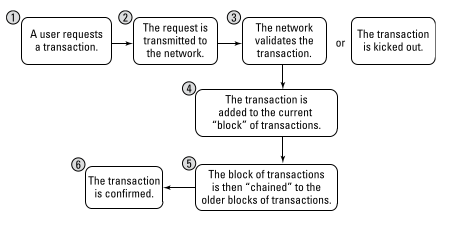
\includegraphics[scale=0.7]{figuras/capitulo_2/blockchain_come_to_agreement.png}
                     \caption{Funcionamento do Blockchain - Imagem retirada de \cite{blockchain_for_dummies}.}
                     \label{fig:blockchain_work_dummies}
                \end{figure}
        
        Os mecanismos de consenso vêm da teoria dos jogos. Os sistemas devem ser projetados de tal forma que os nós obtenham o maior benefício se eles seguirem as regras. Um dos aspectos para garantir que os nós se comportem honestamente é recompensar o comportamento honesto e punir por atividades fraudulentas. No entanto em um blockchain público como o do Bitcoin, um nó pode ter muitas identidades públicas diferentes e anônimas. Fica muito difícil punir essas identidades porque elas têm a opção de evitar essa punição criando novas identidades para si mesmas. Por outro lado, recompensá-los funciona muito bem, porque mesmo que alguém tenha múltiplas identidades, eles podem colher os frutos que lhes são dados \cite{beginnig_blockchain_bikramaditya}.
        
        O objetivo do consenso é também garantir que a rede seja robusta o suficiente para sustentar vários tipos de ataques. Independentemente dos tipos de algoritmos de consenso que um pode escolher, dependendo do caso de uso, ele deve cair no molde de um consenso tolerante a falhas bizantinas para ser aceito \cite{beginnig_blockchain_bikramaditya}.
        
        
        \subsubsection{Protocolos de consenso}

            A escolha do protocolo de consenso afeta a segurança e a escalabilidade. Uma vez que um novo bloco é gerado por um \textit{miner}, o \textit{miner} propaga o bloco para seus pares conectados na rede blockchain. No entanto, os \textit{miners} podem encontrar novos blocos competidores diferentes e resolver isso usando os mecanismos de consenso do blockchain \cite{architecture_for_blockchain}.
            
            A abordagem geral típica é chamada de consenso Nakamoto. Essa abordagem depende dos participantes que selecionam como autoritativa a maior cadeia de blocos que observaram em cada ponto no tempo. No Bitcoin, novos blocos são gerados através de um mecanismo de prova de trabalho (\textit{Proof Of Work}). A prova de trabalho usa um quebra-cabeça criptográfico que é fácil de verificar, mas é difícil de resolver e toma um tempo efetivamente aleatório. Os mineradores de Bitcoin competem para resolver esse quebra-cabeça para cada bloco, usando grandes quantidades de computações (e, portanto, de eletricidade) para aumentar suas chances de vencer a competição pelo bloco. O investimento requerido pelas mineradoras para isso serve para alinhar seus incentivos com o bom funcionamento do sistema como um todo. Existem vários mecanismos de prova de trabalho, como o Ethash 11 usado pelo Ethereum e o Hashcash 12 usado pelo Bitcoin \cite{architecture_for_blockchain}.
            
            A prova de participação (\textit{Proof of stake}) é um mecanismo alternativo para o consenso Nakamoto, que seleciona o próximo nó de mineração com base no controle da moeda digital nativa da rede blockchain. Por exemplo, os mineradores em Peercoin 14 precisam provar a propriedade de uma certa quantia de moeda de Peercoin para os blocos de mineração. Assim, a prova de participação naturalmente alinha os incentivos dos detentores de moeda digital no blockchain com o bom funcionamento do blockchain. Existem vários protocolos de prova de participação, por ex. Tendermint 15 usado em Eris e Casper 16 para Ethereum. Comparado com a prova de trabalho, a prova de participação é mais eficiente em termos de custo, porque muito menos poder computacional é usado na mineração e a latência também é menor \cite{architecture_for_blockchain}.
            
            PBFT é o acrônimo para o algoritmo de Tolerância de Falha Bizantina Prática e é um dos muitos algoritmos de consenso que se pode considerar para uso em um blockchain, embora seja um algoritmo que não é usado para gerar recompensas de mineração. O funcionamento interno do PBFT, em um alto nível, é transmitido para todos os nós participantes que possuem suas próprias réplicas ou estados internos. Quando os nós recebem uma solicitação, eles executam o cálculo com base em seus estados internos. O resultado da computação é então compartilhado com todos os outros nós no sistema. Então, todo nó está ciente do que outros nós estão computando. Considerando seus próprios resultados de computação, juntamente com os recebidos de outros nós, eles tomam uma decisão e se comprometem com um valor final, que é novamente compartilhado entre os nós. Neste momento, cada nó está ciente da decisão final de todos os outros nós. Em seguida, todos respondem com suas decisões finais e, com base na maioria, o consenso final é alcançado.O PBFT pode ser eficiente em comparação com outros algoritmos de consenso, com base no esforço necessário. No entanto, o anonimato no sistema pode ser comprometido devido à maneira como esse algoritmo é projetado \cite{beginnig_blockchain_bikramaditya}.

    
    \subsection{Smart Contracts}
        
        Um cientista de computação e especialista em criptografia chamado Nick Szabo é creditado por desenvolver o conceito de um contrato inteligente. Ele definiu um contrato inteligente como ``um conjunto de promessas, especificadas em formato digital, incluindo protocolos nos quais as partes cumprem essas promessas''. \cite{smart_contracts_szabo}

        Assim, um contrato inteligente é um algoritmo computadorizado, que executa os termos do contrato. No entanto, essa definição não diferencia contratos inteligentes de algumas construções contratuais já bem conhecidas que implementam o desempenho automatizado (desempenho que não depende de intervenções externas para que um conjunto de atividades sejam executadas) em seu funcionamento como máquinas de venda automática. Máquinas de venda automática são definidas como máquinas automáticas independentes que distribuem bens ou prestam serviços quando as moedas são inseridas ou o pagamento por, digamos, um cartão de crédito é feito. Máquinas de venda automática são programadas com certas regras e executadas por essas regras. \cite{blockchain_pratical_guide}
        
        Se não houver uma diferença principal entre as máquinas de venda automática e os contratos inteligentes, os contratos inteligentes são tão antigos quanto a própria lei romana. No primeiro século AC, um engenheiro e matemático grego, Heron de Alexandria, documentou a primeira máquina de venda automática. Sua máquina aceitava uma moeda de dracma e depois distribuia água benta em templos da região. Portanto, os contratos inteligentes, por si só, não são novos \cite{blockchain_pratical_guide}.
        

      %  \cite{bitcoin_and_blockchainsecurity}


\section{Ethereum}


A intenção do Ethereum é fundir e melhorar o conceitos de scripting, altcoins e meta-protocolos on-chain, e permitir que os desenvolvedores criem aplicativos arbitrários baseados em consenso que tenham escalabilidade, padronização, funcionalidade completa, facilidade de desenvolvimento e interoperabilidade oferecidas por esses diferentes paradigmas, simultaneamente. A Ethereum faz isso construindo o que é essencialmente a última camada fundacional abstrata: um blockchain com uma linguagem de programação Turing-completa integrada, permitindo que qualquer um escreva contratos inteligentes e aplicativos descentralizados onde possam criar suas próprias regras arbitrárias de propriedade, formatos de transação e funções de transição de estado \cite{ethereum_white_paper}.

No Ethereum as chamadas “mensagens” se assemelham as transações no Bitcoin, porém com algumas diferenças. Primeiramente, uma mensagem Ethereum pode ser criada por uma entidade externa (usuário) ou por um contrato; segundo, existe uma opção explícita para as mensagens conterem dados; a terceira diferença é que o receptor de uma mensagem Ethereum tem a opção de responder, ou seja, as mensagens ethereunm englobam o conceito de funções \cite{ethereum_white_paper}.

Um contrato inteligente no Ethereum é uma caixa protegida criptograficamente que contém lógica e valor. A lógica tem condições específicas que precisam ser atendidas para liberar o valor. É a adição de lógica e estado que torna o Ethereum uma plataforma mais poderosa do que a que está disponível com outras criptomoedas, incluindo o Bitcoin (e sua funcionalidade de script). Um exemplo de um contrato inteligente para uma empresa de seguros poderia ser utilizado para pagar automaticamente para a entidade segurada com base em um feed de dados que mostrassem que um evento pagável ocorreu.\cite{blockchain_pratical_guide}

Contratos inteligentes permitem aplicativos descentralizados (Dapps). Aplicativos centralizados são serviços realmente centralizados. Por exemplo, quando interagimos com um aplicativo de terceiros em nosso \textit{smartphone}, o aplicativo se comunicará com servidores e serviços centralizados. Um Dapp pode ser exatamente o mesmo em termos da interface do usuário, mas os serviços de \textit{back-end} são substituídos por contratos inteligentes que são executados na rede Ethereum descentralizada \cite{blockchain_pratical_guide}.

O mecanismo de contrato descrito acima permite que qualquer pessoa construa o que é essencialmente um aplicativo de linha de comando executado em uma máquina virtual que é executada por consenso em toda a rede, permitindo modificar um estado globalmente acessível como seu “disco rígido”.
No entanto, para a maioria das pessoas, a interface de linha de comando que é o mecanismo de envio de transações não é suficientemente amigável ao usuário para tornar a descentralização uma alternativa convencional atraente. Para este fim, uma aplicação descentralizada completa deve consistir em
componentes lógicos de negócios de baixo nível, implementados inteiramente na plataforma Ethereum, usando uma combinação de Ethereum e outros sistemas (por exemplo, uma camada de mensagens P2P), e componentes gráficos de interface de usuário de alto nível. O design do cliente Ethereum serve como um navegador da \textit{Web}, mas inclui suporte para um objeto de API JavaScript “eth”, que páginas especificas da \textit{Web} visualizadas no cliente poderão usar para interagir com o blockchain Ethereum. Do ponto de vista da \textit{web} “tradicional”, essas páginas são inteiramente de conteúdo estático, uma vez que o blockchain e outros protocolos descentralizados servirão como um substituto completo do servidor com a finalidade de manipular solicitações iniciadas pelo usuário \cite{ethereum_white_paper}.


\subsection{Aplicações Descentralizadas (Dapp)}

Um aplicativo descentralizado (Dapp) é como qualquer outro aplicativo moderno arquitetado pela Web, geralmente consistindo em uma interface com o usuário (UI) cuja funcionalidade é suportada pelos serviços de \textit{back-end} (leitura e gravação em armazenamento persistente, processamento, lógica complexa). Esses serviços de \textit{back-end} geralmente utilizam a plataforma Ethereum e, em particular, os contratos inteligentes que são implantados para ela. Em retrospecto, pode-se dizer que de certa forma o primeiro Dapp conhecido foi o Bitcoin, porém este não foi implementado na plataforma Ethereum \cite{blockchain_pratical_guide}.

A Figura \ref{fig:dapp_ethereum} representa um exemplo da estrutura de um aplicativo descentralizado.

    \begin{figure}[h]
         \centering
         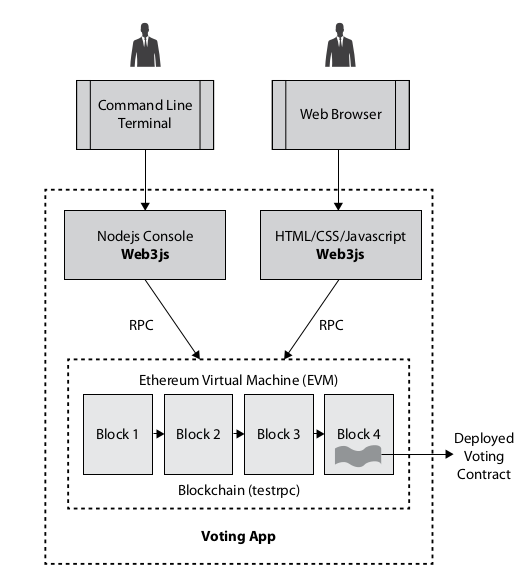
\includegraphics[scale=0.5]{figuras/capitulo_2/ethereum_dapp_structure.png}
         \caption{Aplicação Descentralizada Ethereum - Imagem retirada de \cite{blockchain_pratical_guide}.}
         \label{fig:dapp_ethereum}
    \end{figure}